
We are now going to reimplement the previous neural network with the Keras framework. Keras is an open source neural network library written in Python. It has the advantage of abstracting most of the boiler-plate code one needs to write when implementing a neural net only with a linear algebra library. Thus, it is suitable to fast prototyping and experimentation.

\subsection{Some section with code}

\begin{lstlisting}[language=Python]
    import numpy as np
     
    def incmatrix(genl1,genl2):
        m = len(genl1)
        n = len(genl2)
        M = None #to become the incidence matrix
        VT = np.zeros((n*m,1), int)  #dummy variable
     
        #compute the bitwise xor matrix
        M1 = bitxormatrix(genl1)
        M2 = np.triu(bitxormatrix(genl2),1) 
     
        for i in range(m-1):
            for j in range(i+1, m):
                [r,c] = np.where(M2 == M1[i,j])
                for k in range(len(r)):
                    VT[(i)*n + r[k]] = 1;
                    VT[(i)*n + c[k]] = 1;
                    VT[(j)*n + r[k]] = 1;
                    VT[(j)*n + c[k]] = 1;
     
                    if M is None:
                        M = np.copy(VT)
                    else:
                        M = np.concatenate((M, VT), 1)
     
                    VT = np.zeros((n*m,1), int)
     
        return M
\end{lstlisting}

Code Output

\begin{lstlisting}
    array([[ 0.01,  0.01,  0.01, ...,  1.  ,  0.01,  0.01],
        [ 0.01,  0.01,  1.  , ...,  0.01,  0.01,  0.01],
        [ 0.01,  1.  ,  0.01, ...,  0.01,  0.01,  0.01],
        ..., 
        [ 0.01,  0.01,  0.01, ...,  0.01,  0.01,  0.01],
        [ 0.01,  0.01,  0.01, ...,  0.01,  0.01,  0.01],
        [ 0.01,  0.01,  0.01, ...,  0.01,  0.01,  0.01]])
\end{lstlisting}

\subsection{Section where we add a figure}

\begin{figure}[H]
    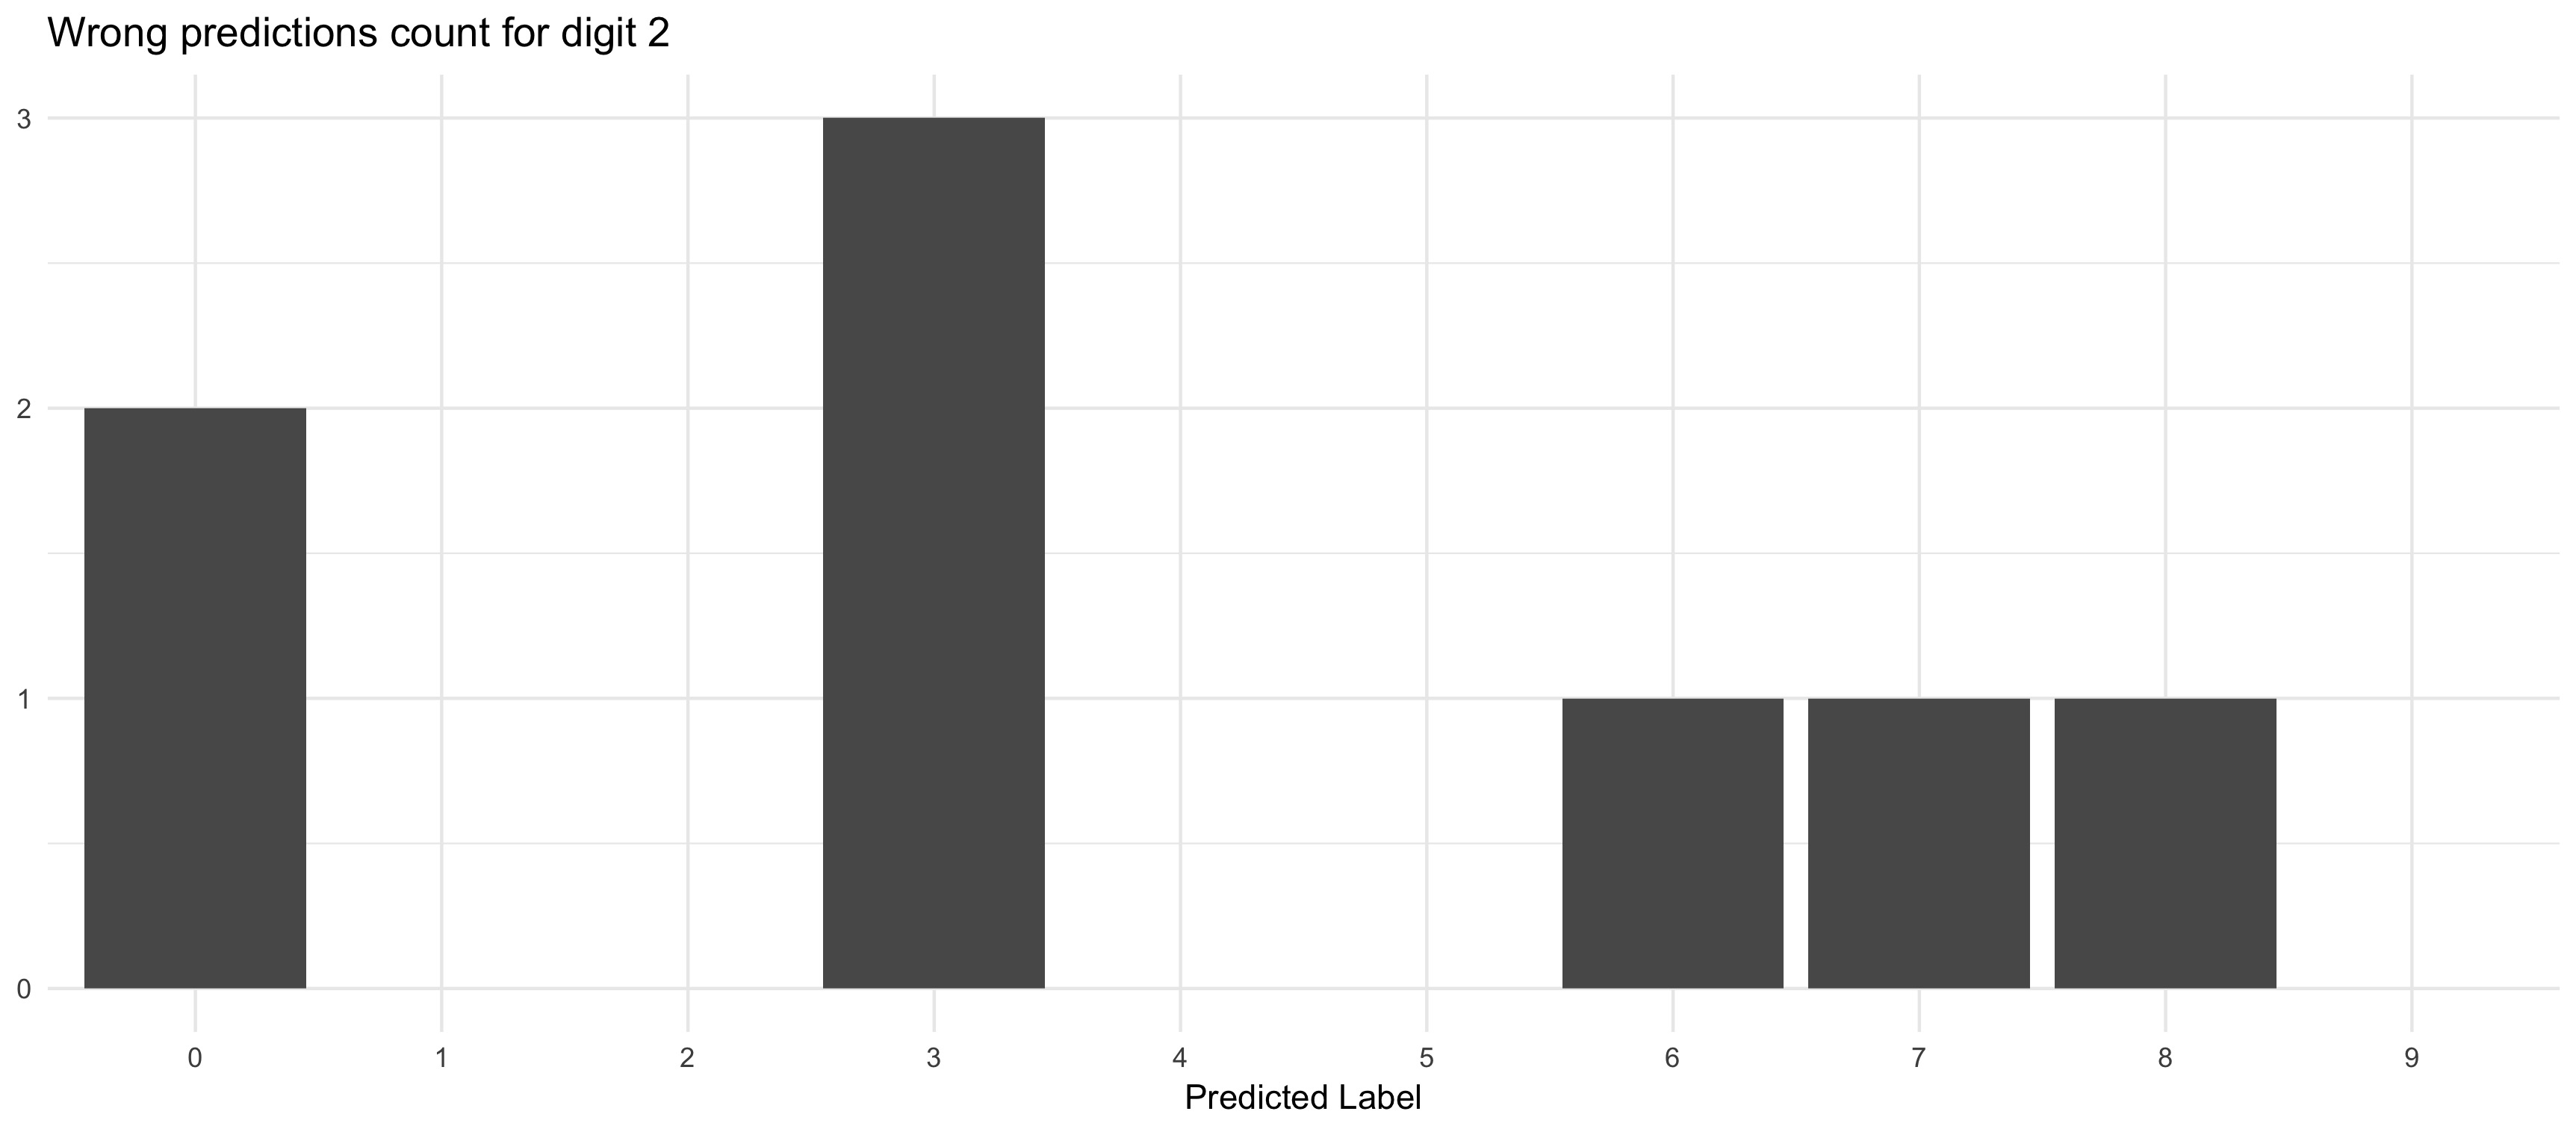
\includegraphics[width=\linewidth]{img/wrong_predictions.jpeg}
    \centering
    \caption{Wrong Predtictions}
    \label{fig:wrong-predictions}
\end{figure}

Figure \ref{fig:wrong-predictions} is very nice.

\begin{equation}
    \int E=m \beta
\end{equation}